\documentclass{report}
\usepackage{graphicx, tikz-cd, float, titlepic, booktabs} % Required for inserting images
\usepackage{pgfplots}
\pgfplotsset{compat=1.15}
\usepackage{mathrsfs}
\usetikzlibrary{arrows}
\usepackage{amsmath, amssymb, amsthm, amsfonts, siunitx, physics, gensymb}
\AtBeginDocument{\RenewCommandCopy\qty\SI}
\usepackage[version=4]{mhchem}
\usepackage[most,many,breakable]{tcolorbox}
\usepackage{xcolor, fancyhdr, varwidth}
\usepackage[Glenn]{fncychap}
%Options: Sonny, Lenny, Glenn, Conny, Rejne, Bjarne, Bjornstrup
\usepackage{hyperref, cleveref}
\usepackage{icomma, enumitem} %comma as decimal and continue enumerate with [resume]
\usepackage[danish]{babel}
%%%%%%%%%%%%%%%%%%%%%%%%%%%%%%
% SELF MADE COLORS
%%%%%%%%%%%%%%%%%%%%%%%%%%%%%%
\definecolor{myg}{RGB}{56, 140, 70}
\definecolor{myb}{RGB}{45, 111, 177}
\definecolor{myr}{RGB}{199, 68, 64}
\definecolor{mytheorembg}{HTML}{F2F2F9}
\definecolor{mytheoremfr}{HTML}{00007B}
\definecolor{mylenmabg}{HTML}{FFFAF8}
\definecolor{mylenmafr}{HTML}{983b0f}
\definecolor{mypropbg}{HTML}{f2fbfc}
\definecolor{mypropfr}{HTML}{191971}
\definecolor{myexamplebg}{HTML}{F2FBF8}
\definecolor{myexamplefr}{HTML}{88D6D1}
\definecolor{myexampleti}{HTML}{2A7F7F}
\definecolor{mydefinitbg}{HTML}{E5E5FF}
\definecolor{mydefinitfr}{HTML}{3F3FA3}
\definecolor{notesgreen}{RGB}{0,162,0}
\definecolor{myp}{RGB}{197, 92, 212}
\definecolor{mygr}{HTML}{2C3338}
\definecolor{myred}{RGB}{127,0,0}
\definecolor{myyellow}{RGB}{169,121,69}
\definecolor{myexercisebg}{HTML}{F2FBF8}
\definecolor{myexercisefg}{HTML}{88D6D1}
%%%%%%%%%%%%%%%%%%%%%%%%%%%%%%%%%%%%%%%%%%%%%%%%%%%%%%%%%%%%%%%%%%%%%%
% Box environments for theorems and problems
%%%%%%%%%%%%%%%%%%%%%%%%%%%%%%%%%%%%%%%%%%%%%%%%%%%%%%%%%%%%%%%%%%%%%
\setlength{\parindent}{1cm}
%================================
% Question BOX
%================================
\makeatletter
\newtcbtheorem{question}{Opgave}{enhanced,
	breakable,
	colback=white,
	colframe=myb!80!black,
	attach boxed title to top left={yshift*=-\tcboxedtitleheight},
	fonttitle=\bfseries,
	title={#2},
	boxed title size=title,
	boxed title style={%
			sharp corners,
			rounded corners=northwest,
			colback=tcbcolframe,
			boxrule=0pt,
		},
	underlay boxed title={%
			\path[fill=tcbcolframe] (title.south west)--(title.south east)
			to[out=0, in=180] ([xshift=5mm]title.east)--
			(title.center-|frame.east)
			[rounded corners=\kvtcb@arc] |-
			(frame.north) -| cycle;
		},
	#1
}{def}
\makeatother
%================================
% DEFINITION BOX
%================================

\newtcbtheorem[]{Definition}{Definition}{enhanced,
	before skip=2mm,after skip=2mm, colback=red!5,colframe=red!80!black,boxrule=0.5mm,
	attach boxed title to top left={xshift=1cm,yshift*=1mm-\tcboxedtitleheight}, varwidth boxed title*=-3cm,
	boxed title style={frame code={
					\path[fill=tcbcolback]
					([yshift=-1mm,xshift=-1mm]frame.north west)
					arc[start angle=0,end angle=180,radius=1mm]
					([yshift=-1mm,xshift=1mm]frame.north east)
					arc[start angle=180,end angle=0,radius=1mm];
					\path[left color=tcbcolback!60!black,right color=tcbcolback!60!black,
						middle color=tcbcolback!80!black]
					([xshift=-2mm]frame.north west) -- ([xshift=2mm]frame.north east)
					[rounded corners=1mm]-- ([xshift=1mm,yshift=-1mm]frame.north east)
					-- (frame.south east) -- (frame.south west)
					-- ([xshift=-1mm,yshift=-1mm]frame.north west)
					[sharp corners]-- cycle;
				},interior engine=empty,
		},
	fonttitle=\bfseries,
	title={#2},#1}{def}
\newtcbtheorem[]{definition}{Definition}{enhanced,
	before skip=2mm,after skip=2mm, colback=red!5,colframe=red!80!black,boxrule=0.5mm,
	attach boxed title to top left={xshift=1cm,yshift*=1mm-\tcboxedtitleheight}, varwidth boxed title*=-3cm,
	boxed title style={frame code={
					\path[fill=tcbcolback]
					([yshift=-1mm,xshift=-1mm]frame.north west)
					arc[start angle=0,end angle=180,radius=1mm]
					([yshift=-1mm,xshift=1mm]frame.north east)
					arc[start angle=180,end angle=0,radius=1mm];
					\path[left color=tcbcolback!60!black,right color=tcbcolback!60!black,
						middle color=tcbcolback!80!black]
					([xshift=-2mm]frame.north west) -- ([xshift=2mm]frame.north east)
					[rounded corners=1mm]-- ([xshift=1mm,yshift=-1mm]frame.north east)
					-- (frame.south east) -- (frame.south west)
					-- ([xshift=-1mm,yshift=-1mm]frame.north west)
					[sharp corners]-- cycle;
				},interior engine=empty,
		},
	fonttitle=\bfseries,
	title={#2},#1}{def}

\newtcbtheorem{theo}%
    {Theorem}{}{theorem}
\newtcolorbox{prob}[1]{colback=red!5!white,colframe=red!50!black,fonttitle=\bfseries,title={#1}}
%================================
% NOTE BOX
%================================

\usetikzlibrary{arrows,calc,shadows.blur}
\tcbuselibrary{skins}
\newtcolorbox{note}[1][]{%
	enhanced jigsaw,
	colback=gray!20!white,%
	colframe=gray!80!black,
	size=small,
	boxrule=1pt,
	title=\textbf{Note:},
	halign title=flush center,
	coltitle=black,
	breakable,
	drop shadow=black!50!white,
	attach boxed title to top left={xshift=1cm,yshift=-\tcboxedtitleheight/2,yshifttext=-\tcboxedtitleheight/2},
	minipage boxed title=1.5cm,
	boxed title style={%
			colback=white,
			size=fbox,
			boxrule=1pt,
			boxsep=2pt,
			underlay={%
					\coordinate (dotA) at ($(interior.west) + (-0.5pt,0)$);
					\coordinate (dotB) at ($(interior.east) + (0.5pt,0)$);
					\begin{scope}
						\clip (interior.north west) rectangle ([xshift=3ex]interior.east);
						\filldraw [white, blur shadow={shadow opacity=60, shadow yshift=-.75ex}, rounded corners=2pt] (interior.north west) rectangle (interior.south east);
					\end{scope}
					\begin{scope}[gray!80!black]
						\fill (dotA) circle (2pt);
						\fill (dotB) circle (2pt);
					\end{scope}
				},
		},
	#1,
}
%================================
% EXAMPLE BOX
%================================
\newtcbtheorem[number within=section]{Example}{Example}
{%
	colback = myexamplebg
	,breakable
	,colframe = myexamplefr
	,coltitle = myexampleti
	,boxrule = 1pt
	,sharp corners
	,detach title
	,before upper=\tcbtitle\par\smallskip
	,fonttitle = \bfseries
	,description font = \mdseries
	,separator sign none
	,description delimiters parenthesis
}
{ex}
%================================
% THEOREM BOX
%================================

\tcbuselibrary{theorems,skins,hooks}
\newtcbtheorem[number within=section]{Theorem}{Theorem}
{%
	enhanced,
	breakable,
	colback = mytheorembg,
	frame hidden,
	boxrule = 0sp,
	borderline west = {2pt}{0pt}{mytheoremfr},
	sharp corners,
	detach title,
	before upper = \tcbtitle\par\smallskip,
	coltitle = mytheoremfr,
	fonttitle = \bfseries\sffamily,
	description font = \mdseries,
	separator sign none,
	segmentation style={solid, mytheoremfr},
}
{th}

%%%%%%%%%%%%%%%%%%%%%%%%%%%%%%%%%%%%%%%%%%%%%%%%%%%%%%%%%%%%%%%%%
% SELF MADE COMMANDS
%%%%%%%%%%%%%%%%%%%%%%%%%%%%%%
\newcommand{\sol}{\setlength{\parindent}{0cm}\textbf{\textit{Løsning:}}\setlength{\parindent}{1cm}}
%%%%%%%%%%%%%%%%%%%%%%%%%%%%%%%%%
\usepackage[tmargin=2cm,rmargin=1in,lmargin=1in,margin=0.85in,bmargin=2cm,footskip=.2in]{geometry}\pagestyle{fancy}
\lhead{Minrui Kevin Zhou 3.b}
\rhead{Rapport 1: Oxidation af butanolerne}

\title{Rapport 1: Oxidation af butanolerne\\
{\Large \textbf{3.b kemi A}}}
\author{Kevin Zhou}
\date{\today}
\titlepic{\includegraphics[width=0.7\textwidth]{pipette_hånd.jpg}}
\begin{document}
\maketitle
\section*{Formål}
Formålet med eksperimentet er at forsøge på at oxidere de fire butanoler og ved at undersøge oxidationsprodukterne bestemme, om de hver især er primære, sekundære eller tertiære alkoholer.
\section*{Teori}
Det er i eksperimentet relevant at kunne skelne mellem primære, sekundære og tertiære alkoholer.
Disse betegnelser er ret intuitive, idet man ser på, om det \ce{C}-atom, som \ce{OH}-gruppen sidder på er primært, sekundært eller tertiært (det kan åbenlyst ikke være kvartært).
Altså vil det sige, at \ce{OH}-gruppen sidder på et endestillet \ce{C}-atom i en primær alkohol, og at i en tertiær alkohol sidder \ce{OH}-gruppen på et \ce{C}-atom, der er bundet til tre andre \ce{C}-atomer.

Det er værd at tilføje, at primære og sekundære alkoholer kan oxideres ved brug af milde oxidationsmidler, hvor der ved tertiære alkoholer virkeligt skal udøves vold.
Primære alkoholer oxideres til aldehyder, der yderligere kan oxideres til carboxylsyrer.
Sekundære alkoholer oxideres til ketoner, der ikke yderligere kan oxideres.

De fire alkholer med molekylformlen \ce{C4H9OH} kalder vi for de fire butanoler.
Strukturformlerne for disse ses i \cref{fig:butanoler}.
De systematiske navne for de fire alkoholer er henholdsvis butan-1-ol, butan-2-ol, 2-methylpropan-1-ol og 2-methylpropan-2-ol.
Ved at se på strukturformlerne er det klart, at butan-1-ol og 2-methylpropan-1-ol er primære alkoholer, hvor butan-2-ol er sekundær og 2-methylpropan-2-ol er tertiær.
\begin{figure}[H]
\begin{center}
  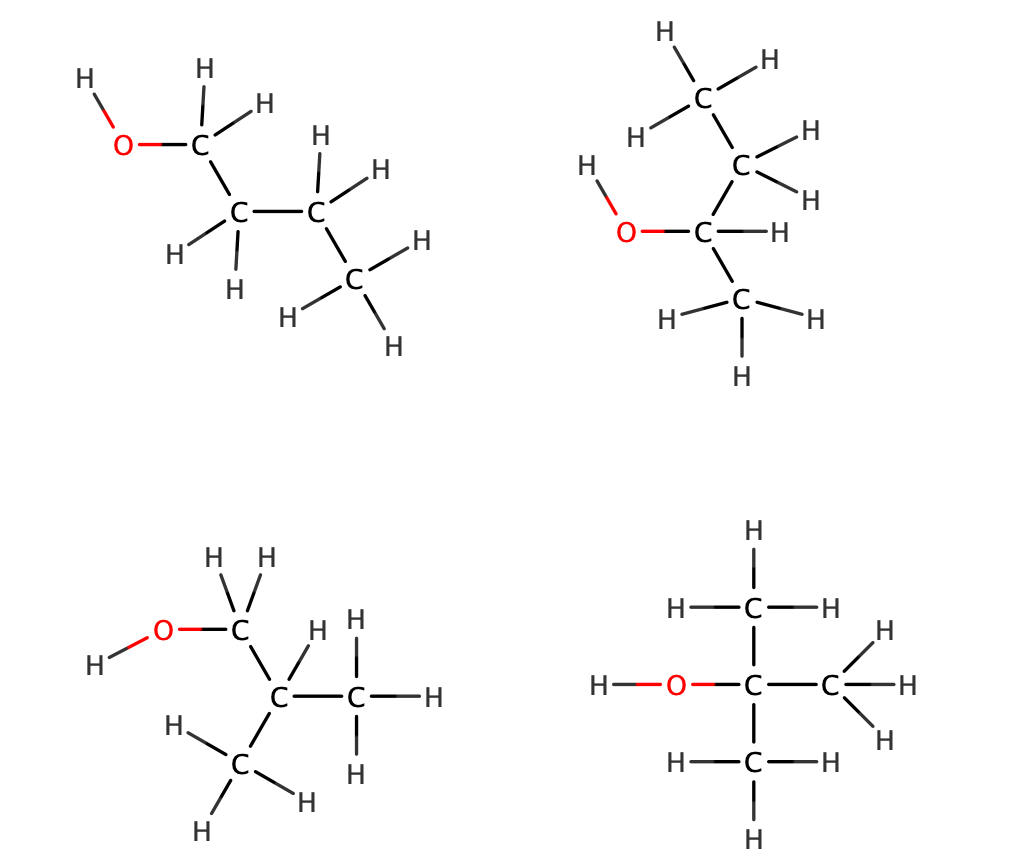
\includegraphics[scale=0.45]{butanoler.png}
\end{center}
\caption{Strukturformler for de fire isomere butanoler tegnet i MarvinSketch}
\label{fig:butanoler}
\end{figure}
I eksperimentet oxideres alkoholerne med den violette permanganat, \ce{MnO4-}, i sur opløsning.
Den uafstemte redoxreaktion for oxidationen af en primær alkohol kan ses i \cref{eq:redox}, hvor $R$ betegner et radikal. 
\begin{equation}
\label{eq:redox}
\begin{split}
  \ce{R-CH2OH + \underset{\text{violet} }{\ce{MnO4-}} ->T[sur] R-CHO + \underset{\text{farveløs}}{\ce{Mn^2+} }}
\end{split}
\end{equation}
Denne redoxreaktion kan nemt afstemmes ved at se bort fra radikalet, da der ikke sker nogen ændring i denne gruppe ved reaktionen.
Dette ses i \cref{fig:redox}.
\begin{figure}[H]
\begin{center}
  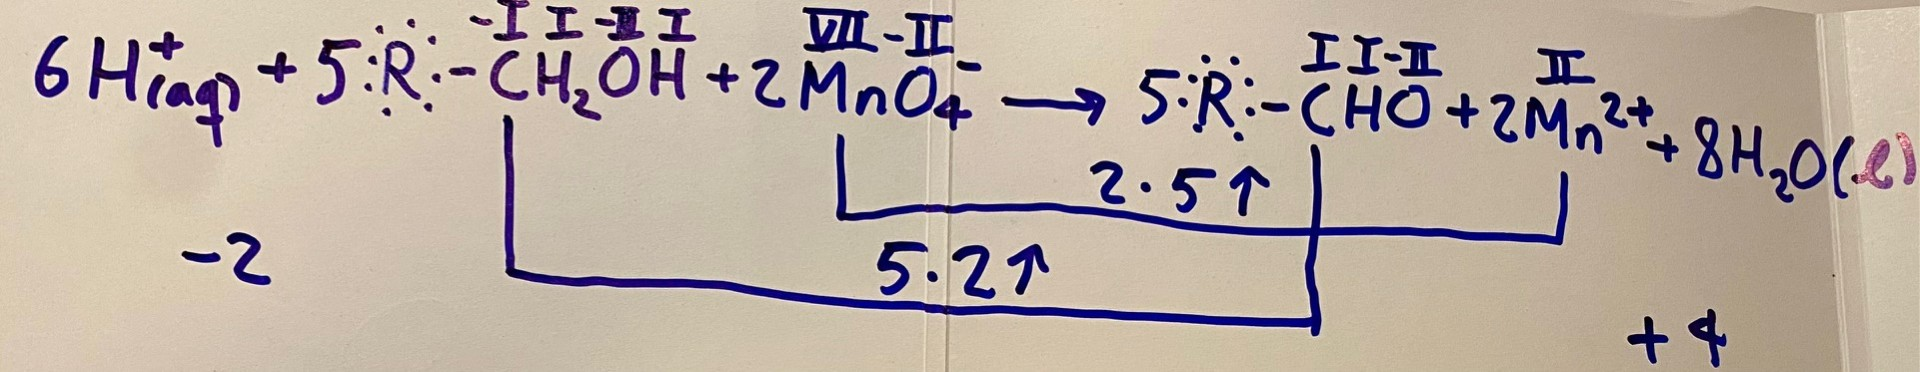
\includegraphics[scale=0.3]{redox.jpg}
\end{center}
\caption{Redoxreaktionen afstemt i hånden}
\label{fig:redox}
\end{figure}

\section*{Apparatur, kemikalier og sikkerhed}
\subsection*{Apparatur}
\begin{itemize}
  \item Minireagensglas
  \item Reagensglasstativ
\item Bunsenbrænder
\item Trefod med trådnet
\item Bægerglas, $100 \;\unit{mL} $
\item Plastpipetter
\end{itemize}
\subsection*{Kemikalier}
\begin{itemize}
  \item $0,4 \;\unit{\textsc{m}} $ \ce{KMnO4} (ca. mættet opløsning)
\item 2,4-dinitrophenylhydrazin-opløsning
\item $0,05 \;\unit{\textsc{m}} $ \ce{AgNO3}-opløsning
\item $2 \;\unit{\textsc{m}} $ \ce{H2SO4}  
\item $2 \;\unit{\textsc{m}} $ \ce{NaOH} 
\item $2 \;\unit{\textsc{m}} $ \ce{NH3} 
\item De fire butanoler fordelt i hver sin flaske mærket A, B, C og D
\end{itemize}
\subsection*{Sikkerhed}
\begin{itemize}
  \item $2 \;\unit{\textsc{m}} $ \ce{H2SO4}, $2 \;\unit{\textsc{m}} $ \ce{NaOH} og $2 \;\unit{\textsc{m}} $ \ce{NH3} virker ætsende.
 \item $0,4 \;\unit{\textsc{m}} $ \ce{KMnO4} og $0,05 \;\unit{\textsc{m}} $ \ce{AgNO3} virker ætsende og giver sorte pletter på hud og tøj.
\item Opløsningen af 2,4-dinitrophenylhydrazin virker ætsende og er farlig ved hudkontakt, indåndning og indtagelse.
\item Alkoholerne er brandfarlige og farlige ved hudkontakt, indånding og indtagelse. 
\end{itemize}

\section*{Udførelse}
Et $100 \;\unit{mL} $ bægerglas fyldes halvt op med demineraliseret vand og varmes op på en trefod over en bunsenbrænder indtil vandet næsten koger.

Til fire reagensglas tilsættes hver 5 dråber 2,4-dinitrophenylhydrazin-opløsning. Disse stilles i et reagensglasstativ. 
Herefter tilsættes fire nye reagensglas hver 5 dråber $0,05 \;\unit{\textsc{m}} $ \ce{AgNO3}, 1 dråbe $2 \;\unit{\textsc{m}} $ \ce{NaOH} og så hurtigt 4 dråber $2 \;\unit{\textsc{m}} $ \ce{NH3}. 
De omrystes forsigtigt ved at knipse på glasset, og tilsættes lidt mere $2 \;\unit{\textsc{m}} $ \ce{NH3}, dersom det brune bundfald ikke opløses. 
Disse fire reagensglas stilles ligeledes i reagensglasstativet.

De fire butanoler undersøges herefter en ad gangen.
Først afmåles i et rent reagnesglas 8 dråber $0,4 \;\unit{\textsc{m}} $ \ce{KMnO4} og 5 dråber $2 \;\unit{\textsc{m}} $ \ce{H2SO4}, hvorefter 5 dråber af den undersøgte alkohol tilsættes.
Reagensglasset omrystes forsigtigt.

Reagensglasset opvarmes så i vandbadet, hvor tydelige farveskift i reaktionsblandingen observeres.

Når glassets indhold er varmt, stikkes en ren plastpipette ned i glasset uden at røre væsken. 
Dampe pumpes ind og ud af pipetten nogle gange, så muligt fordampet reaktionsprodukt suges ind i pipetten.
Dette kan ses i \cref{fig:hånd_pipette}.
\begin{figure}[H]
\begin{center}
  \includegraphics[scale=0.5]{pipette_hånd.jpg}
\end{center}
\caption{Muligt fordampet reaktionsprodukt suges ind i pipetten}
\label{fig:hånd_pipette}
\end{figure}
Pipetten stikkes så ned i et af glassene med 2,4-dinitrophenylhydrazin uden at ramme væsken og pumpes forsigtigt nogle gange med forsigtig omrystning.
Der observeres så, om der kommer et gult bundfald eller en tydelig uklarhed i opløsningen.

Mere damp suges hurtigt herefter op i pipetten (også som i \cref{fig:hånd_pipette}), og pumpes ud i et af reagensglassene med Tollens reagens mens det omrystes forsigtigt.
Der observeres om der kommer et sølvspejl eller sort bundfald som i \cref{fig:sort_pipette}.
Denne process gentages for alle fire butanoler.
\begin{figure}[H]
\begin{center}
  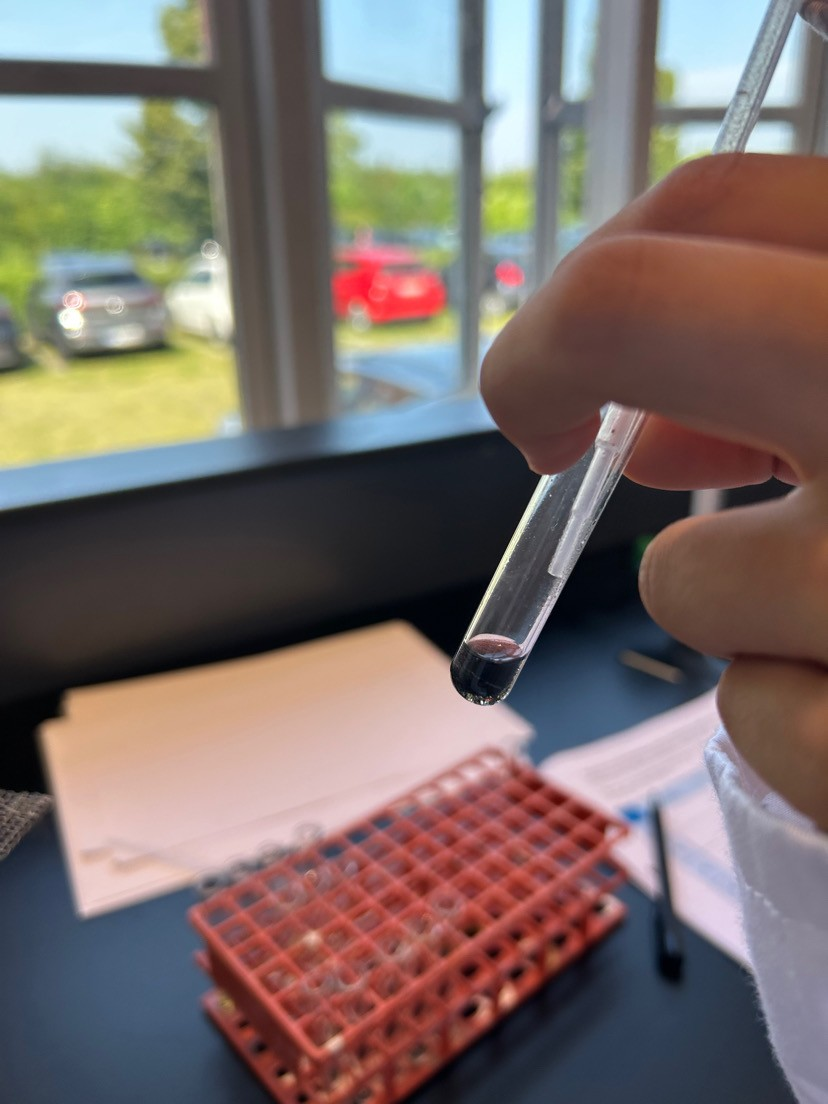
\includegraphics[scale=0.5]{sort_pipette.jpg}
\end{center}
\caption{Fordampet oxidationsprodukt pumpes ned i reagensglas med Tollens reagens}
\label{fig:sort_pipette}
\end{figure}

\section*{Resultater}
Observationerne ved undersøgelse af hver af de fire butanoler ses i tabel \ref{tab:observationer}.
Bemærk at ved observation med 2,4-dnp og med Tollens er tale om reaktionen med \textit{oxidationsproduktet}.
\begin{table}[H]
\centering
\begin{tabular}{@{}llll@{}}
\toprule
Alkohol & Observation ved oxidation & Observation med 2,4-dnp & Observation med Tollens \\ \midrule
A       & bliver farveløs           & orange bundfald         & sort bundfald           \\
B       & -                         & -                       & -                       \\
C       & bliver farveløs           & orange bundfald         & -                       \\
D       & bliver farveløs           & orange bundfald         & sort bundfald           \\ \bottomrule
\end{tabular}
\caption{Observationer ved undersøgelse af de fire alkoholer}
\label{tab:observationer}
\end{table}

\section*{Efterbehandling og sammenfatning}
Fra \cref{eq:redox} ser vi, at farveskift ved oxidationsforsøget fortæller, om der er sket en oxidation eller ej.
Altså bliver blandingen mere farveløs og mindre violet, hvis der sker en oxidation, da $[\ce{MnO4-}]$ bliver mindre. 

Testen med 2,4-dinitrophenylhydrazin bruges til at afgøre, om oxidationsproduktet er en carbonylforbindelse.
Hvis det er tilfældet, dannes et orange bundfald.

Testen med Tollens' reagens bruges til at afgøre, om oxidationsproduktet er en aldehyd, da aldehyder, men ikke ketoner reagerer med Tollens' reagens.

Vi kan da med resultaterne fra tabel \ref{tab:observationer} udlede resultaterne i tabel \ref{tab:kon}.
Hvis der dannes bundfald både ved testen med 2,4-dnph og Tollens, så må oxidationsproduktet være en aldehyd.
Dette kan kun lade sig gøre, hvis alkoholen er primær og er tilfældet for alkohol A og D.
Hvis hverken dannes bundfald ved testen med 2,4-dnph og Tollens samtidig med, at der ikke er farveskift ved oxidationsforsøget, er det da tydeligt, at ingen oxidation sker.
Altså må alkoholen være tertiær, hvilket er tilfældet for alkohol B.
Hvis der dannes bundfald ved testen med 2,4-dnph, men ikke ved testen med Tollens' reagens, så er oxidationsproduktet en keton.
Altså er alkoholen sekundær, hvilket er tilfældet for alkohol C.
\begin{table}[H]
\centering
\begin{tabular}{@{}clccc@{}}
\toprule
\multicolumn{1}{l}{Alkohol} & Oxideres alkoholen? & \multicolumn{1}{l}{Er ox.-produktet en carbonyl-forb.?} & \multicolumn{1}{l}{Er ox.-produktet en aldehyd?} & \multicolumn{1}{l}{Konklusion} \\ \midrule
A                           & Ja                  & Ja                                                            & Ja                                               & Primær                                    \\
B                           & Nej                 & Nej                                                           & Nej                                              & Tertiær                                   \\
C                           & Ja                  & Ja                                                            & Nej                                              & Sekundær                                  \\
D                           & Ja                  & Ja                                                            & Ja                                               & Primær                                    \\ \bottomrule
\end{tabular}
\caption{Vi kan ud fra resultaterne konkludere om alkoholerne hver især er primære, sekundære eller tertiære}
\label{tab:kon}
\end{table}
Ved at kigge på \cref{fig:butanoler} ser vi, at vores resultater stemmer i overensstemmelse med, at to af de fire alkoholer er primære, én er sekundær og én er tertiær.

\section*{Mulige fejlkilder}
Ved oxidationen af alkoholen er det vigtigt, at man hurtigt fjerner oxidationsproduktet fra reaktionsblandingen, da aldehyder, som primære alkoholer oxideres til, kan oxideres videre til carboxylsyrer, der hverken kan reagere med 2,4-dinitrophenylhydrazin eller Tollens' reagens.
Derudover kan man også risikere, at oxidationsprodukterne kan slippe væk.

\section*{Konklusion}
Vi har altså oxideret de fire butanoler (aktuelt set kun tre), hvorefter vi har bestemt alkohol A og D til at være primære, B til at være tertiær og C til at være sekundær.
Dette er i overensstemmelse med, at to af de fire butanoler er primære, en er sekundær og en er tertiær.

\end{document}
